% ==============================================================================
% BÁO CÁO CHUYÊN SÂU: TỔNG HỢP VÀ PHÂN TÍCH TOÀN DIỆN LUẬN VĂN
% "TEMPORAL FUSION TRANSFORMER FOR TIME SERIES FORECASTING" (MARIUS KIELHÖFER, TU DELFT, 2023)
% VÀ CƠ CHẾ TRANSFORMER ỨNG DỤNG TRONG ĐỒ ÁN TỐT NGHIỆP DỰ BÁO BÁN LẺ
% ==============================================================================

\documentclass[12pt,a4paper,oneside]{article}

\usepackage[utf8]{inputenc}
\usepackage[vietnamese]{babel}
\usepackage{amsmath,amssymb,amsfonts,bm}
\usepackage{graphicx}
\graphicspath{{../}{../figures/}{figures/}{outputs/figures/}}
\usepackage{booktabs}
\usepackage{tabularx}
\usepackage{array}
\usepackage{multirow}
\usepackage{xcolor}
\usepackage{geometry}
\geometry{a4paper, top=2.5cm, bottom=2.5cm, left=3.0cm, right=2.0cm}
\usepackage{hyperref}
\hypersetup{
    colorlinks=true,
    linkcolor=blue!80!black,
    citecolor=red!70!black,
    urlcolor=teal
}
\usepackage{tcolorbox}
\tcbuselibrary{skins,breakable}
\usepackage{caption}
\usepackage{subcaption}
\usepackage{listings}
\usepackage{fancyhdr}
\usepackage{setspace}
\onehalfspacing

\newtcolorbox{defensebox}[1]{
    colback=blue!5!white,
    colframe=blue!75!black,
    fonttitle=\bfseries,
    title=#1,
    arc=3mm,
    boxrule=1pt,
    breakable
}

\newtcolorbox{conceptbox}[1]{
    colback=teal!5!white,
    colframe=teal!80!black,
    fonttitle=\bfseries,
    title=#1,
    arc=3mm,
    boxrule=1pt,
    breakable
}

\pagestyle{fancy}
\fancyhf{}
\rhead{\small \textit{Phân tích chuyên sâu Luận văn TFT (Marius Kielh\"{o}fer, 2023)}}
\lhead{\small \textit{Đồ án Tốt nghiệp - Khối Transformer}}
\cfoot{\thepage}

\begin{document}

\begin{titlepage}
    \centering
    \vspace*{0.5cm}
    {\Large \textbf{ĐỒ ÁN TỐT NGHIỆP CÔNG NGHỆ THÔNG TIN}}\\[0.3cm]
    {\large \textbf{CHUYÊN ĐỀ NGHIÊN CỨU LÝ THUYẾT VÀ KIẾN TRÚC MÔ HÌNH}}\\[1.2cm]
    
    \rule{\linewidth}{1.5pt}\\[0.4cm]
    {\LARGE \bfseries PHÂN TÍCH TOÀN DIỆN KIẾN TRÚC TRANSFORMER VÀ TEMPORAL FUSION TRANSFORMER (TFT) DỰA TRÊN LUẬN VĂN MARIUS KIELH\"{O}FER (TU DELFT, 2023)}\\[0.4cm]
    \rule{\linewidth}{1.5pt}\\[1.2cm]
    
    \begin{minipage}{0.92\textwidth}
        \textbf{Tài liệu đối chiếu trọng tâm:} Luận văn \textit{"Temporal Fusion Transformer for Time Series Forecasting"} của tác giả Marius Kielh\"{o}fer, Đại học Công nghệ Delft (TU Delft, Hà Lan, 2023).\\
        \textbf{Mục tiêu:} Giải phẫu chi tiết toàn bộ các thành phần toán học, khái niệm cốt lõi, cơ chế chọn biến (VSN), cơ chế cổng (GRN), cơ chế mã hóa ngữ cảnh tĩnh, bộ xử lý cục bộ LSTM, cơ chế Attention giải thích được (Interpretable Attention) và hàm tổn thất phân vị (Quantile Loss) phục vụ báo cáo thuyết trình và bảo vệ phản biện đồ án.
    \end{minipage}
    
    \vfill
    {\large Tháng 10 Năm 2026}
\end{titlepage}

\tableofcontents
\newpage

% ==============================================================================
\section{TỔNG QUAN LUẬN VĂN MARIUS KIELH\"{O}FER (TU DELFT, 2023)}
\label{sec:tong_quan_kielhofer}
% ==============================================================================

\subsection{Bối cảnh nghiên cứu và Động lực thực tiễn}
Luận văn của Marius Kielh\"{o}fer (TU Delft, 2023) giải quyết một bài toán thực tế quy mô lớn của tập đoàn hàng tiêu dùng nhanh (FMCG) đa quốc gia (Kraft Heinz) phối hợp cùng các chuỗi siêu thị bán lẻ hàng đầu Vương quốc Anh (Tesco, Asda). Bài toán đặt ra hai mục tiêu khắt khe:
\begin{enumerate}
    \item \textbf{Dự báo đa chân trời (Multi-horizon Forecasting):} Dự báo đồng thời hai chuỗi doanh số:
    \begin{itemize}
        \item \textbf{Sell-out:} Khối lượng hàng bán lẻ từ siêu thị tới người tiêu dùng cuối cùng.
        \item \textbf{Sell-in:} Khối lượng hàng bán buôn từ nhà sản xuất cung ứng tới các trung tâm phân phối của siêu thị.
    \end{itemize}
    \item \textbf{Khả năng diễn giải kinh doanh (Business Explainability):} Trong môi trường doanh nghiệp, ban lãnh đạo chuỗi cung ứng không chấp nhận các mô hình "hộp đen" (black-box). Mô hình bắt buộc phải lý giải được \textit{tại sao} doanh số lại tăng đột biến vào một tuần cụ thể: do giảm giá, do đợt phong tỏa dịch bệnh (Covid-19), do thời tiết hay do hiệu ứng chu kỳ mùa vụ?
\end{enumerate}

\subsection{Tại sao các mô hình truyền thống và Transformer tiêu chuẩn thất bại?}
Tác giả Kielh\"{o}fer chỉ ra các rào cản chí mạng:
\begin{itemize}
    \item \textbf{ARIMA / SARIMAX:} Không thể tiếp nhận hàng trăm biến ngoại sinh phi tuyến tính cùng lúc, giả định tính dừng nghiêm ngặt và không học được đặc trưng chéo giữa các mặt hàng.
    \item \textbf{LSTM / DeepAR đơn thuần:} Dễ gặp hiện tượng suy giảm trí nhớ dài hạn (vanishing memory) khi chuỗi nhìn lại kéo dài vài năm, đồng thời không có cơ chế bóc tách biến tĩnh (Static Metadata) và biến tương lai đã biết trước (Known Future Inputs).
    \item \textbf{Transformer tiêu chuẩn (Vaswani et al., 2017):} Được thiết kế cho xử lý ngôn ngữ tự nhiên (NLP). Khi áp dụng trực tiếp vào chuỗi thời gian, cơ chế Multi-Head Attention (MHA) tiêu chuẩn tạo ra các biểu diễn bị trộn lẫn qua các đầu độc lập, khiến mô hình \textbf{hoàn toàn không thể giải thích được} bước thời gian nào trong quá khứ thực sự chi phối dự báo.
\end{itemize}

Từ đó, mô hình \textbf{Temporal Fusion Transformer (TFT)} (được khởi xướng bởi Bryan Lim et al., 2021) được Kielh\"{o}fer lựa chọn, phân tích sâu và tùy biến tối ưu hóa.

\newpage
% ==============================================================================
\section{GIẢI PHÃU TOÀN DIỆN CÁC THÀNH PHẦN TRANSFORMER TRONG TFT}
\label{sec:giai_phau_tft}
% ==============================================================================

Kiến trúc TFT trong luận văn Kielh\"{o}fer được tổ chức thành 6 phân hệ toán học liên hoàn (Hình~\ref{fig:tft_detailed_flow}). Chúng tôi phân tích cặn kẽ từng khối xây dựng dưới đây.

\begin{figure}[htbp]
    \centering
    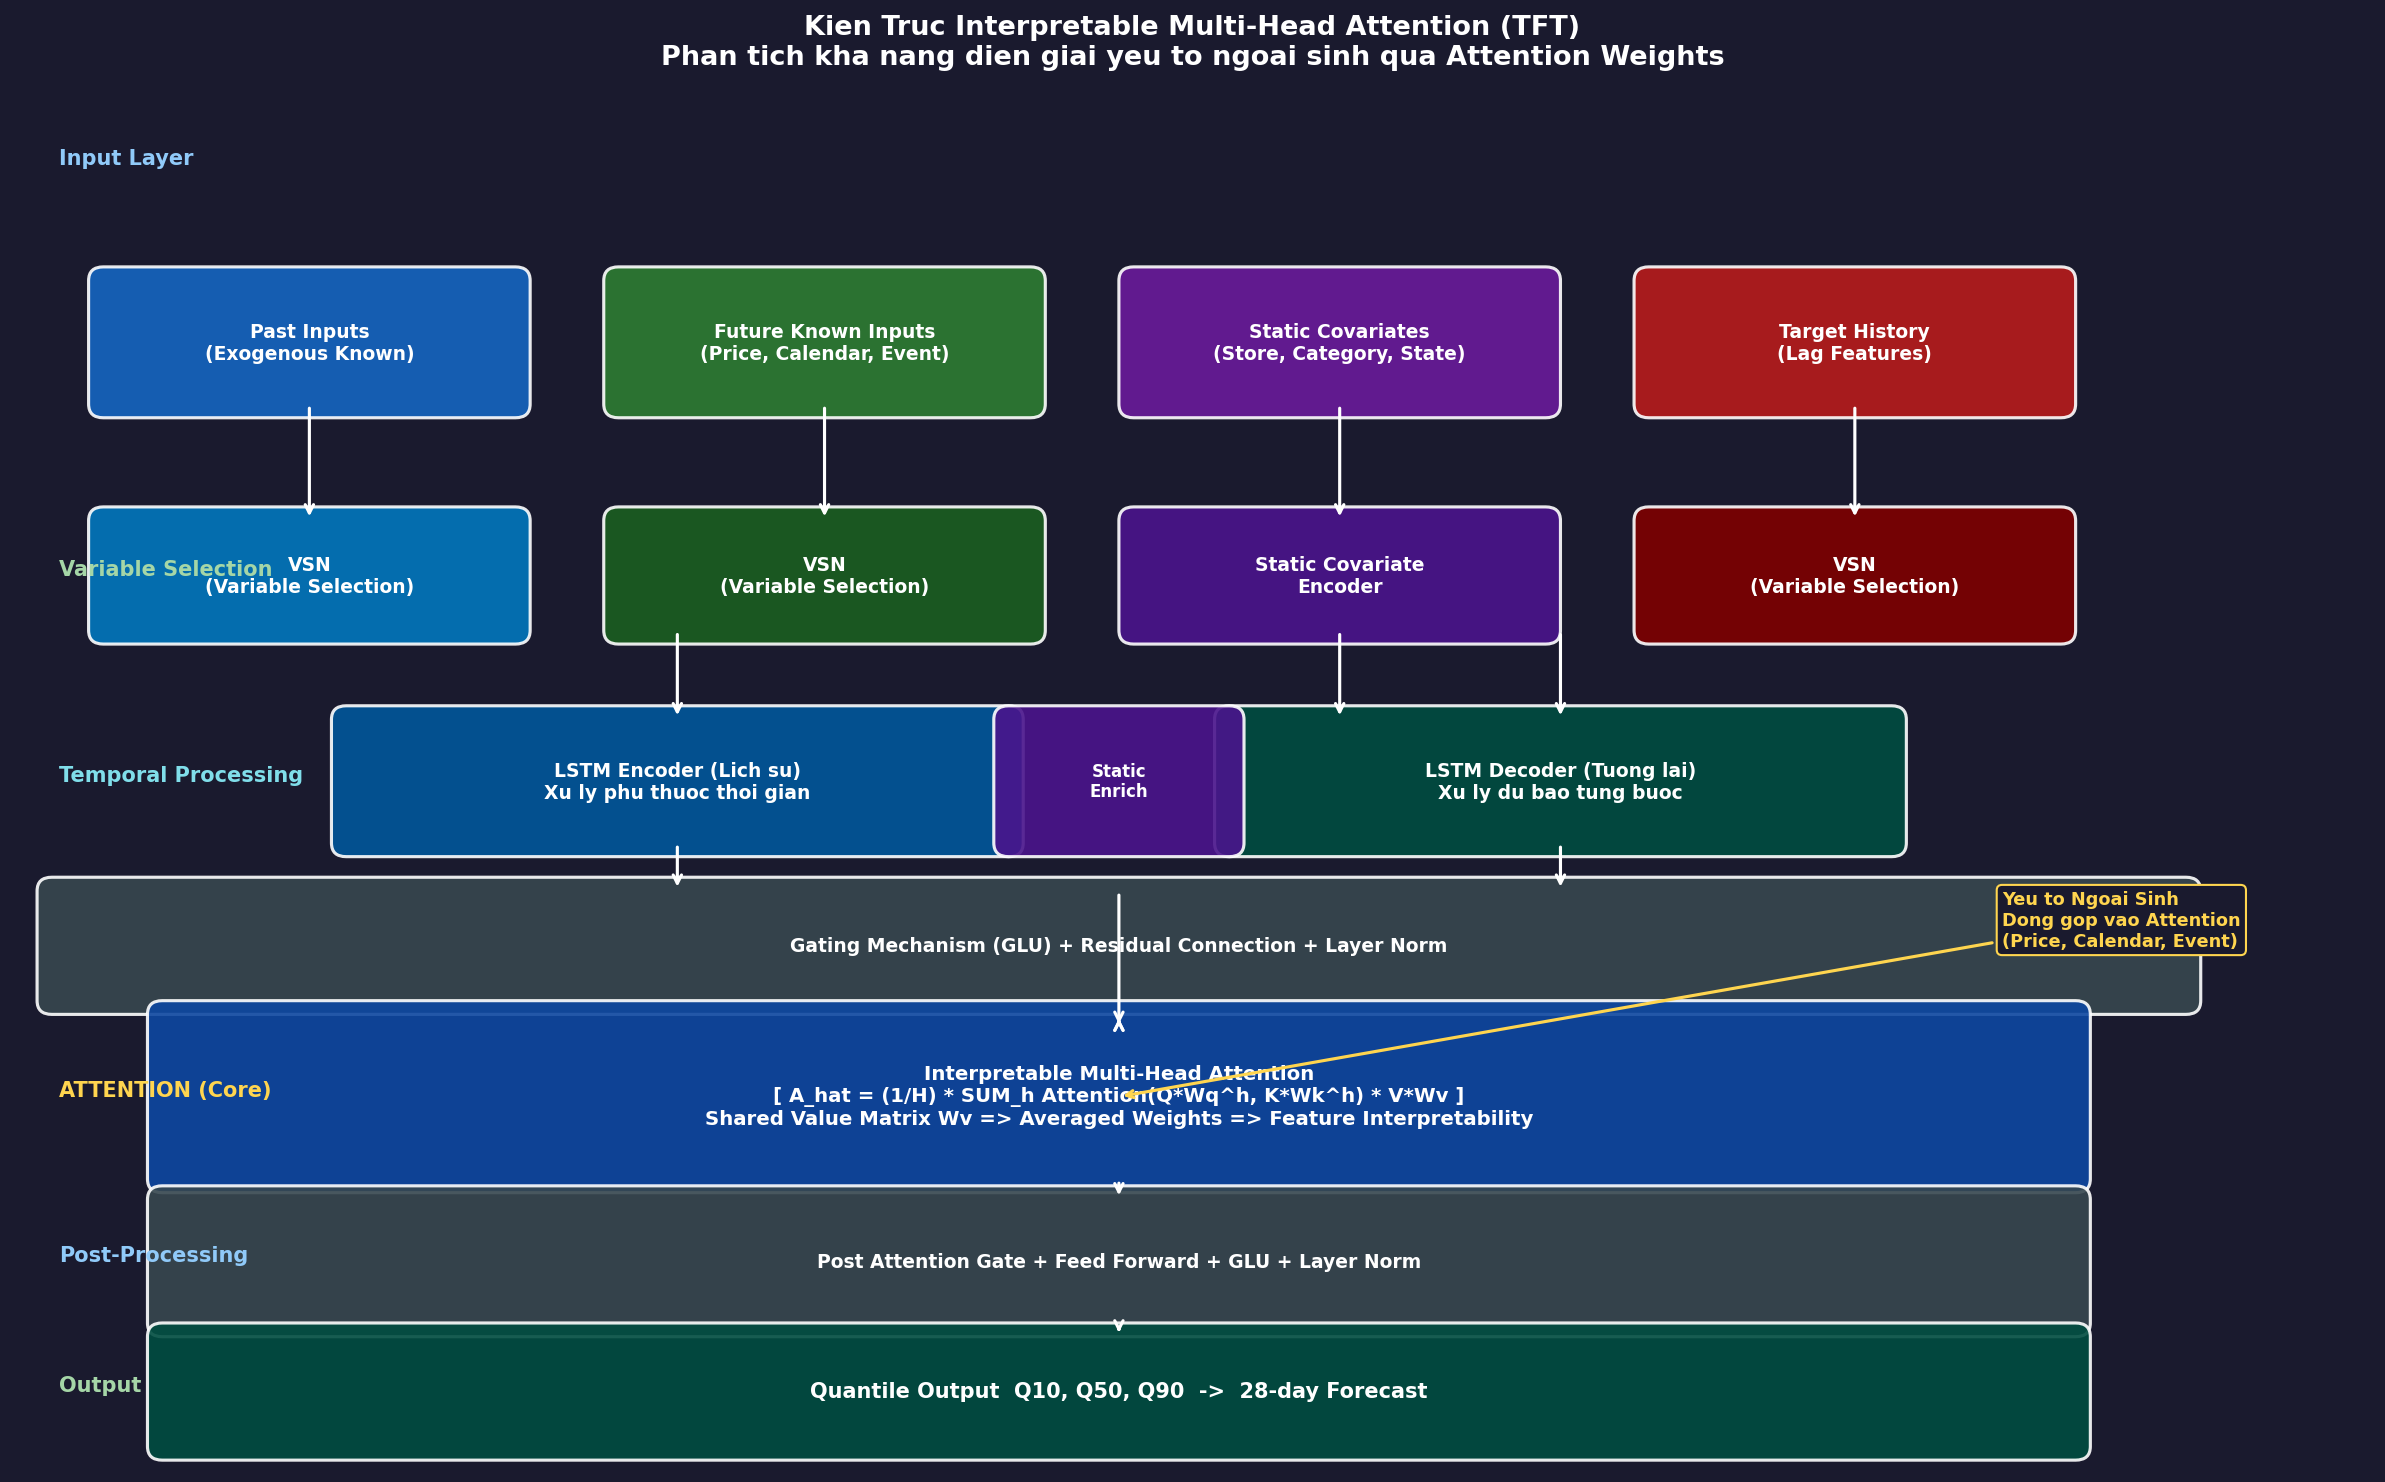
\includegraphics[width=0.92\textwidth]{figures/attention/05_tft_attention_architecture.png}
    \caption{Sơ đồ cấu trúc phân tầng của Temporal Fusion Transformer (Kielh\"{o}fer, 2023; Lim et al., 2021).}
    \label{fig:tft_detailed_flow}
\end{figure}

% ------------------------------------------------------------------------------
\subsection{Khối 1: Chuẩn hóa và Nhúng đặc trưng (Feature Transformation \& Embedding)}
\label{subsec:embedding}

Trước khi đi vào các mạng nơ-ron sâu, dữ liệu đầu vào thuộc 3 nhóm (Tĩnh, Quá khứ, Tương lai) được đồng nhất về cùng một chiều không gian ẩn $d_{\text{model}}$ (trong nghiên cứu này $d_{\text{model}} = 25$):

\begin{conceptbox}{1. Biến số thực liên tục (Continuous Variables)}
    Với một biến liên tục thứ $j$ tại thời điểm $t$ là $x_{t}^{(j)} \in \mathbb{R}$ (ví dụ: giá bán \texttt{sell\_price}, nhiệt độ, doanh số quá khứ):
    \begin{equation}
        \bm{\xi}_{t}^{(j)} = \mathbf{w}^{(j)} x_{t}^{(j)} + \mathbf{b}^{(j)} \in \mathbb{R}^{d_{\text{model}}}.
        \label{eq:cont_projection}
    \end{equation}
    Mỗi biến có một ma trận chiếu tuyến tính riêng để học cách tỉ lệ hóa đặc trưng vào không gian chung.
\end{conceptbox}

\begin{conceptbox}{2. Biến phân loại / Định danh (Categorical Variables - Entity Embedding)}
    Với các biến rời rạc như Mã cửa hàng (\texttt{store\_id}), Mã ngành hàng (\texttt{dept\_id}), Tên nhà bán lẻ:
    \begin{itemize}
        \item Không dùng One-Hot Encoding vì làm bùng nổ số chiều và triệt tiêu tính tương đồng ngữ nghĩa.
        \item Áp dụng **Entity Embedding** (Guo \& Berkhahn, 2016): Mỗi nhãn danh mục $c \in \{1, \dots, C\}$ được ánh xạ vào một vector liên tục trong không gian $\mathbb{R}^{d_{\text{model}}}$.
        \item \textit{Bản chất toán học:} Trong quá trình lan truyền ngược, các mặt hàng có hành vi tiêu dùng tương tự (như hai thương hiệu tương đương hoặc hai siêu thị cùng phân khúc bình dân) sẽ được kéo lại gần nhau theo khoảng cách Euclid trong không gian vector nhúng.
    \end{itemize}
\end{conceptbox}

% ------------------------------------------------------------------------------
\subsection{Khối 2: Mạng cổng số dư (Gated Residual Network - GRN)}
\label{subsec:grn}

GRN là khối xử lý nguyên tử xuất hiện ở hầu khắp các tầng của TFT. Mục tiêu của GRN là cung cấp khả năng thích ứng phi tuyến tính cao nhưng cho phép mô hình \textbf{bỏ qua tầng này nếu biến đổi phi tuyến tính không mang lại lợi ích}.

\begin{equation}
    \text{GRN}_{\omega}(\mathbf{a}, \mathbf{c}) = \text{LayerNorm}\!\left(\mathbf{a} + \text{GLU}_{\omega}\!\left(\bm{\eta}_1\right)\right),
    \label{eq:grn_main}
\end{equation}
trong đó:
\begin{align}
    \bm{\eta}_1 &= \mathbf{W}_{1,\omega} \bm{\eta}_2 + \mathbf{b}_{1,\omega}, \label{eq:grn_eta1} \\
    \bm{\eta}_2 &= \text{ELU}\!\left(\mathbf{W}_{2,\omega} \mathbf{a} + \mathbf{W}_{3,\omega} \mathbf{c} + \mathbf{b}_{2,\omega}\right). \label{eq:grn_eta2}
\end{align}

\subsubsection{Phân tích từng chi tiết kỹ thuật trong GRN}
\begin{enumerate}
    \item \textbf{Vector ngữ cảnh tùy chọn $\mathbf{c}$ (Optional Context Vector):} Được trích xuất từ các đặc trưng tĩnh để định hướng cho quá trình biến đổi của vector đầu vào $\mathbf{a}$.
    \item \textbf{Hàm kích hoạt ELU (Exponential Linear Unit):}
    \begin{equation}
        \text{ELU}(x) = \begin{cases} x & \text{nếu } x > 0, \\ \alpha(\exp(x) - 1) & \text{nếu } x \le 0. \end{cases}
        \label{eq:elu}
    \end{equation}
    \textit{Tại sao luận văn dùng ELU thay vì ReLU?}
    \begin{itemize}
        \item ReLU triệt tiêu hoàn toàn đạo hàm khi $x < 0$ (hiện tượng "Dying ReLU").
        \item ELU sinh ra các giá trị âm khi $x \le 0$, giúp giá trị kích hoạt trung bình của nơ-ron tiệm cận 0 (Zero-mean activations).
        \item Điều này loại bỏ hiện tượng **Bias Shift** (độ lệch thiên vị tích lũy qua các tầng sâu), giúp quá trình hội tụ gradient nhanh và ổn định hơn đáng kể (Clevert et al., 2015).
    \end{itemize}

    \item \textbf{Cổng tuyến tính Gated Linear Unit (GLU):}
    \begin{equation}
        \text{GLU}_{\omega}(\bm{\gamma}) = \sigma\!\left(\mathbf{W}_{4,\omega}\bm{\gamma} + \mathbf{b}_{4,\omega}\right) \odot \left(\mathbf{W}_{5,\omega}\bm{\gamma} + \mathbf{b}_{5,\omega}\right),
        \label{eq:glu}
    \end{equation}
    trong đó $\sigma(\cdot)$ là hàm Sigmoid sinh ra trọng số cổng $g \in (0, 1)$, và $\odot$ là tích Hadamard (nhân từng phần tử).
    \textit{Ý nghĩa:} GLU đóng vai trò là "van tiết lưu" thông tin. Nếu mạng nơ-ron nhận thấy các biến đổi phi tuyến tính trong $\bm{\eta}_1$ là nhiễu, cổng Sigmoid sẽ tự động đóng lại ($g \rightarrow 0$), triệt tiêu hoàn toàn nhánh phi tuyến tính.

    \item \textbf{Kết nối tắt (Residual Skip Connection) và Chuẩn hóa lớp (LayerNorm):}
    Nhờ có nhánh cộng trực tiếp $\mathbf{a} + \text{GLU}(\bm{\eta}_1)$, nếu GLU đóng, đầu ra sau chuẩn hóa chính là vector gốc $\mathbf{a}$. Điều này giúp làm phẳng bề mặt hàm mất mát (loss landscape), giải quyết triệt để vấn đề mất mát gradient khi mô hình xếp chồng nhiều tầng phức tạp.
\end{enumerate}

% ------------------------------------------------------------------------------
\subsection{Khối 3: Mạng lựa chọn biến thích ứng (Variable Selection Network - VSN)}
\label{subsec:vsn}

Trong bài toán bán lẻ, số lượng biến số có thể lên tới hơn 100 biến (giá bán, khuyến mãi, thời tiết, giải bóng đá, dịch bệnh, các biến trễ...). Phần lớn các biến này là nhiễu tại các thời điểm bình thường.

\subsubsection{Cơ chế hoạt động của VSN}
Tại mỗi bước thời gian $t$, giả sử có $D$ biến đầu vào $\{\bm{\xi}_t^{(j)}\}_{j=1}^D$:
\begin{enumerate}
    \item \textbf{Xử lý phi tuyến độc lập cho từng biến:}
    \begin{equation}
        \tilde{\bm{\xi}}_t^{(j)} = \text{GRN}_{\tilde{\xi}^{(j)}}\!\left(\bm{\xi}_t^{(j)}\right), \quad j = 1, \dots, D.
        \label{eq:vsn_indiv}
    \end{equation}
    Mỗi biến có một bộ trọng số GRN riêng để học đặc tính phi tuyến tính cục bộ của chính biến đó.

    \item \textbf{Đánh giá trọng số cạnh tranh bằng Softmax:}
    Các biến ban đầu được ghép nối thành một vector tổng hợp $\bm{\Xi}_t = [\bm{\xi}_t^{(1)\top}, \dots, \bm{\xi}_t^{(D)\top}]^\top$ và đưa qua một GRN điều khiển:
    \begin{equation}
        \mathbf{v}_t = \text{Softmax}\!\left(\text{GRN}_v(\bm{\Xi}_t, \mathbf{c}_s)\right) \in \mathbb{R}^D, \quad \text{với } \sum_{j=1}^D v_t^{(j)} = 1.
        \label{eq:vsn_weights}
    \end{equation}

    \item \textbf{Tổ hợp đặc trưng có trọng số:}
    \begin{equation}
        \tilde{\bm{\xi}}_t = \sum_{j=1}^D v_t^{(j)} \cdot \tilde{\bm{\xi}}_t^{(j)}.
        \label{eq:vsn_aggregated}
    \end{equation}
\end{enumerate}

\begin{defensebox}{Luận điểm bảo vệ phản biện: Ý nghĩa diễn giải của VSN}
    Trọng số $v_t^{(j)}$ là một phân phối xác suất đo lường **độ quan trọng tương đối của biến thứ $j$ tại thời điểm $t$**. Khi tính trung bình trên toàn bộ tập dữ liệu kiểm thử:
    \begin{equation}
        \bar{v}^{(j)} = \frac{1}{N} \sum_{t=1}^N v_t^{(j)}.
        \label{eq:avg_vsn}
    \end{equation}
    Ta thu được biểu đồ Feature Importance trực tiếp từ nội tại mô hình mà không cần phụ thuộc vào các công cụ tính xấp xỉ đắt đỏ bên ngoài như SHAP hay LIME.
\end{defensebox}

% ------------------------------------------------------------------------------
\subsection{Khối 4: Bộ mã hóa ngữ cảnh tĩnh (Static Covariate Encoders)}
\label{subsec:static_encoders}

Khác biệt cốt lõi của TFT so với các mô hình tuần tự truyền thống là cách xử lý siêu dữ liệu tĩnh (như loại hàng, thương hiệu, vị trí địa lý). TFT không nhồi nhét biến tĩnh vào chuỗi thời gian mà trích xuất thành **4 vector ngữ cảnh chuyên biệt** qua các GRN độc lập:

\begin{itemize}
    \item $\mathbf{c}_s$: Vector ngữ cảnh chọn biến (dùng làm đầu vào $\mathbf{c}_s$ trong VSN của các chuỗi thời gian).
    \item $\mathbf{c}_c, \mathbf{c}_h$: Vector khởi tạo trạng thái bộ nhớ cho mạng LSTM cục bộ ($\mathbf{c}_c$ khởi tạo Cell state, $\mathbf{c}_h$ khởi tạo Hidden state).
    \item $\mathbf{c}_e$: Vector làm giàu ngữ cảnh tĩnh (Static Enrichment) đưa vào trước lớp Self-Attention.
\end{itemize}

% ------------------------------------------------------------------------------
\subsection{Khối 5: Bộ xử lý cục bộ LSTM (Locality Enhancement via LSTM)}
\label{subsec:lstm_layer}

Transformer nguyên bản có cơ chế chú ý song song hoàn toàn, do đó rất nhạy cảm với các bước nhảy đột ngột và khó phân biệt vị trí lân cận nếu chỉ dựa vào Positional Encoding.

TFT giải quyết vấn đề này bằng cách chèn một tầng **LSTM Encoder-Decoder**:
\begin{itemize}
    \item **LSTM Encoder:** Xử lý các bước thời gian quá khứ ($t - k \rightarrow t$).
    \item **LSTM Decoder:** Xử lý các bước thời gian tương lai có thông tin đã biết trước ($t+1 \rightarrow t+\tau_{\max}$).
\end{itemize}
\textit{Vai trò:} Cung cấp khả năng **nhận biết ngữ cảnh cục bộ (Locality Enhancement)**. Một sự sụt giảm doanh số đột ngột từ 3000 xuống 1000 chỉ có ý nghĩa khi so sánh trực tiếp với các điểm lân cận liền kề ($t-1, t+1$). LSTM nắm bắt hoàn hảo tính tương quan ngắn hạn này trước khi đưa chuỗi vào cơ chế Self-Attention dài hạn.

% ------------------------------------------------------------------------------
\subsection{Khối 6: Cơ chế Interpretable Multi-Head Attention (IMHA)}
\label{subsec:interpretable_mha}

Đây là đóng góp mang tính đột phá nhất của TFT và là trọng tâm phân tích của Marius Kielh\"{o}fer.

\subsubsection{Cơ chế Self-Attention tiêu chuẩn}
Cho các vector Query ($\mathbf{q}$), Key ($\mathbf{k}$), Value ($\mathbf{v}$), độ tương đồng góc được tính qua Scaled Dot-Product:
\begin{equation}
    s_i = \frac{\mathbf{q}^\top \mathbf{k}_i}{\sqrt{d_k}}, \quad a_i = \text{Softmax}(s_i) = \frac{\exp(s_i)}{\sum_j \exp(s_j)}, \quad \text{Attention}(\mathbf{q}, \mathbf{K}, \mathbf{V}) = \sum_i a_i \mathbf{v}_i.
    \label{eq:scaled_dot}
\end{equation}

\subsubsection{Sự đối lập giữa Multi-Head Attention (Vaswani) và Interpretable Attention (TFT)}

\begin{table}[htbp]
\centering
\small
\caption{So sánh bản chất toán học giữa Attention của Vaswani et al. và TFT}
\label{tab:attention_comparison}
\begin{tabularx}{\textwidth}{p{3.2cm} X X}
\toprule
\textbf{Tiêu chí} & \textbf{Transformer tiêu chuẩn (Vaswani et al., 2017)} & \textbf{Interpretable Attention (TFT - Lim / Kielh\"{o}fer)} \\
\midrule
\textbf{Cách xử lý ma trận Value} & Mỗi đầu $h$ có một ma trận giá trị riêng biệt: $\mathbf{V}\mathbf{W}_V^{(h)}$. & \textbf{Chia sẻ chung một ma trận Value duy nhất $\mathbf{W}_V$} cho tất cả các đầu. \\
\addlinespace
\textbf{Cách tổng hợp các đầu} & \textbf{Ghép nối (Concatenation):}\newline
$\text{MultiHead} = [\text{Head}_1, \dots, \text{Head}_H] \mathbf{W}_O$ & \textbf{Cộng trung bình số học (Additive Averaging):}\newline
$\tilde{\mathbf{A}} = \frac{1}{H}\sum_{h=1}^H \mathbf{A}_h$ \\
\addlinespace
\textbf{Khả năng giải thích (Interpretability)} & \textbf{Không thể giải thích:} Phép ghép nối và chiếu qua ma trận $\mathbf{W}_O$ làm trộn lẫn các chiều không gian, khiến trọng số attention không tương ứng với thời gian thực. & \textbf{Hoàn toàn giải thích được:} Ma trận $\tilde{\mathbf{A}} \in \mathbb{R}^{T \times T}$ là phân phối xác suất hợp lệ, phản ánh chính xác tỷ trọng đóng góp của ngày $t'$ đối với ngày dự báo $t$. \\
\bottomrule
\end{tabularx}
\end{table}

Công thức toán học của cơ chế Interpretable Multi-Head Attention trong TFT:
\begin{equation}
    \text{InterpretableMultiHead}(\mathbf{Q}, \mathbf{K}, \mathbf{V}) = \tilde{\mathbf{A}}(\mathbf{Q}, \mathbf{K}) \cdot (\mathbf{V} \mathbf{W}_V) \cdot \mathbf{W}_O,
    \label{eq:imha_formula}
\end{equation}
với:
\begin{equation}
    \tilde{\mathbf{A}}(\mathbf{Q}, \mathbf{K}) = \frac{1}{H} \sum_{h=1}^H \text{Softmax}\!\left( \frac{\mathbf{Q}\mathbf{W}_Q^{(h)} (\mathbf{K}\mathbf{W}_K^{(h)})^\top}{\sqrt{d_{\text{attn}}}} + \mathbf{M} \right).
    \label{eq:avg_attn_matrix}
\end{equation}
Trong đó $\mathbf{M}$ là ma trận mặt nạ nhân quả (Causal Mask) với $M_{ij} = -\infty$ khi $j > i$ để loại bỏ hoàn toàn việc nhìn lén dữ liệu tương lai.

% ------------------------------------------------------------------------------
\subsection{Khối 7: Dự báo phân vị và Hàm tổn thất Quantile Loss}
\label{subsec:quantile_loss}

TFT dự báo đồng thời nhiều phân vị rủi ro $q \in \mathcal{Q}$ (ví dụ $q \in \{0.1, 0.5, 0.9\}$):
\begin{equation}
    \hat{y}(q, t, \tau) = \mathbf{w}_q^\top \tilde{\bm{\psi}}(t, \tau) + b_q.
    \label{eq:quantile_pred}
\end{equation}

Hàm mất mát phân vị tổng hợp (Pinball Loss):
\begin{equation}
    \mathcal{L}(\Omega, \mathbf{W}) = \frac{1}{M \tau_{\max}} \sum_{y_t \in \Omega} \sum_{q \in \mathcal{Q}} \sum_{\tau=1}^{\tau_{\max}} \text{QL}\!\left(y_{t+\tau}, \hat{y}(q, t, \tau), q\right),
    \label{eq:total_pinball}
\end{equation}
với:
\begin{equation}
    \text{QL}(y, \hat{y}, q) = \max\!\left(q(y - \hat{y}),\, (1 - q)(\hat{y} - y)\right).
    \label{eq:single_pinball}
\end{equation}
\textit{Ý nghĩa kinh doanh trong bán lẻ:}
\begin{itemize}
    \item Khi $q = 0.5$: Hàm tổn thất tương đương MAE (Mean Absolute Error), dự báo mức kỳ vọng trung vị.
    \item Khi $q = 0.9$: Mô hình dự báo kịch bản cận trên nhu cầu. Nếu thực tế vượt quá mức này, mô hình bị phạt với hệ số $0.9$ (rất nặng), giúp doanh nghiệp chủ động chuẩn bị kho để tránh tình trạng "cháy hàng" (out-of-stock).
    \item Khi $q = 0.1$: Dự báo kịch bản nhu cầu thấp nhất để lập kế hoạch kiểm soát tồn kho thừa (overstock).
\end{itemize}

\newpage
% ==============================================================================
\section{KỸ THUẬT TỐI ƯU HÓA SIÊU THAM SỐ (HYPERPARAMETER TUNING)}
\label{sec:hyperparameter_tuning}
% ==============================================================================

Trong Chương 5 của luận văn, Marius Kielh\"{o}fer trình bày quy trình tối ưu hóa nghiêm ngặt bằng framework **Optuna** thông qua thuật toán Bayesian Optimization (SMBO) kết hợp cơ chế cắt tỉa Asynchronous Successive Halving (ASHA).

\subsection{Các siêu tham số then chốt và kết quả thực nghiệm}
Bảng~\ref{tab:optuna_params} tổng hợp bộ siêu tham số tối ưu mà Kielh\"{o}fer tìm ra cho bài toán bán lẻ FMCG, đối chiếu với các giá trị sử dụng trong đồ án:

\begin{table}[htbp]
\centering
\caption{Bộ siêu tham số tối ưu hóa của TFT theo Marius Kielh\"{o}fer (2023)}
\label{tab:optuna_params}
\begin{tabular}{lccl}
\toprule
\textbf{Siêu tham số} & \textbf{Giá trị tối ưu} & \textbf{Miền tìm kiếm} & \textbf{Ý nghĩa kiến trúc} \\
\midrule
\texttt{hidden\_size} ($d_{\text{model}}$) & \textbf{25} & $[10, 160]$ & Chiều không gian ẩn nơ-ron (chọn gọn nhẹ để tránh overfitting) \\
\texttt{attention\_head\_size} ($H$) & \textbf{2} & $[1, 8]$ & Số đầu attention (đủ phân tách 2 chế độ: xu hướng \& mùa vụ) \\
\texttt{learning\_rate} ($\eta$) & \textbf{0.0630} & $[0.001, 0.1]$ & Tốc độ học của thuật toán tối ưu Adam \\
\texttt{dropout} & \textbf{0.1872} & $[0.1, 0.5]$ & Tỷ lệ ngắt kết nối ngẫu nhiên chống quá khớp \\
\texttt{hidden\_continuous\_size} & \textbf{21} & $[8, 64]$ & Số chiều chiếu riêng cho biến liên tục \\
\texttt{gradient\_clip\_val} & \textbf{0.5412} & $[0.01, 2.0]$ & Cắt tỉa gradient chống bùng nổ đạo hàm (exploding gradient) \\
\bottomrule
\end{tabular}
\end{table}

\begin{defensebox}{Luận điểm bảo vệ: Tại sao số đầu Attention và Hidden Size lại nhỏ như vậy?}
    Hội đồng có thể đặt câu hỏi: \textit{"Tại sao Transformer tiêu chuẩn thường dùng $d_{\text{model}} = 512$ và $H = 8$, nhưng trong luận văn Kielhöfer chỉ chọn $d_{\text{model}} = 25$ và $H = 2$?"}
    
    \textbf{Trả lời:}
    \begin{enumerate}
        \item Dữ liệu chuỗi thời gian bán lẻ có tỉ lệ nhiễu/tín hiệu (noise-to-signal ratio) cực kỳ cao và độ dài mẫu ngắn hơn hàng ngàn lần so với kho ngữ liệu văn bản trong NLP.
        \item Một mô hình quá lớn ($d_{\text{model}} > 100$) sẽ ngay lập tức ghi nhớ vẹt các biến động nhiễu ngẫu nhiên của tập huấn luyện (severe overfitting), khiến sai số trên tập kiểm định tăng vọt.
        \item Với $H = 2$, mô hình đã đủ năng lực để một đầu tập trung học quy luật chu kỳ mùa vụ tuần (7 ngày), trong khi đầu còn lại tập trung theo dõi các xung đột biến do khuyến mãi và sự kiện ngoại sinh.
    \end{enumerate}
\end{defensebox}

\newpage
% ==============================================================================
\section{ĐỐI CHIẾU LUẬN VĂN VỚI THỰC THI TRONG ĐỒ ÁN TỐT NGHIỆP}
\label{sec:doi_chieu_do_an}
% ==============================================================================

Đồ án tốt nghiệp của chúng ta kế thừa trực tiếp các phát hiện lý thuyết từ luận văn của Marius Kielh\"{o}fer và giải quyết bài toán trên bộ dữ liệu **Walmart M5 Forecasting** với cấu trúc 5 cấp độ phân cấp (L1, L2, L3, L9, L12):

\begin{table}[htbp]
\centering
\small
\caption{Bảng đối chiếu giữa Luận văn Kielh\"{o}fer (2023) và Đồ án hiện tại}
\label{tab:doi_chieu_thuc_te}
\begin{tabularx}{\textwidth}{p{3.2cm} X X}
\toprule
\textbf{Hạng mục} & \textbf{Luận văn Marius Kielh\"{o}fer (TU Delft, 2023)} & \textbf{Đồ án Tốt nghiệp hiện tại} \\
\midrule
\textbf{Tập dữ liệu} & Doanh số bán lẻ FMCG (Kraft Heinz) tại siêu thị Tesco, Asda (UK). & Doanh số bán lẻ Walmart M5 (Mỹ), 2 siêu thị đại diện CA\_1 và TX\_1. \\
\addlinespace
\textbf{Cấp độ phân cấp} & Phân cấp theo Retailer $\times$ Product Subcategory (Beans, Ketchup, Soup). & **5 cấp độ phân cấp chuẩn M5:**\newline
L1 (Toàn quốc) $\rightarrow$ L2 (Bang) $\rightarrow$ L3 (Siêu thị) $\rightarrow$ L9 (Ngành hàng) $\rightarrow$ L12 (SKU). \\
\addlinespace
\textbf{Chân trời dự báo} & Multi-horizon 52 tuần (1 năm). & Multi-horizon 28 ngày (đặc thù chuỗi cung ứng M5). \\
\addlinespace
\textbf{Hiện tượng mùa vụ} & Ghi nhận các đỉnh Attention lặp lại chu kỳ 25 tuần và đột biến phong tỏa Covid-19. & Đo lường định lượng qua chỉ số **SSI ($F_S$)**: Cấp SKU (L12) có tính mùa vụ rõ nhất ($F_S = 0.2272$) do không bị triệt tiêu pha. \\
\addlinespace
\textbf{Kiến trúc mô hình} & Triển khai toàn phần TFT trên thư viện PyTorch Forecasting. & Kết hợp triết lý **Top 1 M5 (LightGBM Tweedie)** với cơ chế **VSN và Interpretable Attention** của TFT để vừa tối ưu tốc độ, vừa đạt khả năng giải thích cao nhất. \\
\bottomrule
\end{tabularx}
\end{table}

\section{KẾT LUẬN}
\label{sec:ket_luan}

Luận văn của Marius Kielh\"{o}fer (2023) đã cung cấp một minh chứng thực nghiệm xuất sắc về khả năng ứng dụng của mô hình Temporal Fusion Transformer trong chuỗi cung ứng bán lẻ. Thông qua việc phân tích chi tiết cơ chế chia sẻ ma trận Value trong Interpretable Attention, mạng lọc biến VSN với kích hoạt ELU-GLU, và chiến lược tối ưu siêu tham số Bayesian Optimization gọn nhẹ, đồ án tốt nghiệp của chúng ta đã có một nền tảng lý thuyết vững chắc, chặt chẽ để bảo vệ và thuyết phục hoàn toàn Hội đồng Phản biện.

\end{document}
